\chapter{Sprint 3}\label{cha:sprint3}
This sprint aims to explore the possibilities of building our own tracking system as well as updating the RESTful intermediate service to finally fulfil the goals from \cref{cha:sprint2} and resolve issues. Furthermore, we will examine our system in regards to the aspect of security.

\section{Intermediate Server Update}\label{sec:proxy_update1}
We plan on implementing an update to the intermediate server that is used to communicate with Aalborg University's MSE. This update is a consequence of MSE being updated to support geographic coordinates. The update is planned to remove a bug causing loss of data during conversion between different data formats. This section covers the motivation for the following changes in the update:

\begin{itemize}
\item Resolved loss of data during conversion
\item Obfuscates new data acquired as a result of aforementioned change
\item The service no longer stops if it loses its connection with MSE
\item Now checks if MSE is online, and whether the right account information is received, at start-up
\item Supports paging
\end{itemize}

\subsection{Loss of Data}
Geographical coordinates are now supported by MSE, thanks to the MSE administrator at Aalborg University. To perform obfuscation of personal sensitive data, we can convert the returned string to classes containing all information in its member variables. With this method we can easily perform obfuscation of the data we are disallowed to keep by editing the fields corresponding to the personal sensitive data.

This method utilizes a library developed by Google called gson \cite{gson}, which affords the ability to convert strings of the JSON format to a Java class and vice versa. We can acquire the classes by using an online tool called jsonschema2pojo \cite{jsonschematwopojo}, that analyses JSON strings and automatically generates classes with corresponding fields.

Initially, the generated classes did not contain fields for the global coordinates, as they were based on the response string from a version of MSE where this feature was disabled. This would not be a problem for a single conversion, as the generated classes have a field called \textit{additionalProperties}, which contains additional information that could store the coordinates. However, in order to preserve the transparency of the intermediate server, we wish to perform a conversion back to JSON in order to maintain the external illusion of this intermediate server being an MSE service.

Performing several conversions results in a loss of data, as any information in the additionalProperties field is lost. To avoid this data loss, we can re-generate the classes using a JSON string with the appropriate information. Alternatively, we could perform a string search for specific keywords in the JSON string, which we would then obfuscate. However, search and replace in strings is undesirable, in particular because the JSON string often is more than a million characters long. The class of strings in Java is immutable, meaning any changes to a string variable results in new memory being allocated and the modified content of the old memory location copied over. Performing replacements in a large string is very expensive, and it is as such desirable to perform the aforementioned class conversions. 

As a result of the update we now receive specific information that were previously unattainable through the MSE developer test system. This information includes personal sensitive data, which is now being obfuscated when necessary needed. 

\subsection{Connectivity with MSE}
After the initial deployment of the service we experienced downtime as a result of MSE being under maintenance. This was an unexpected event, and as such the program reacted in an unforeseen fashion. Part of the update integrates elements from the client, described in \ref{sec:fetch_data}, in an effort to increase robustness and as such uptime of the service. As a result, the service now sends an initial request to MSE, to confirm the MSE IP address and account info. Furthermore, the service is able to handle MSE being unresponsive.

\subsection{Paging}
When requesting all clients from MSE the response is partitioned into pages. Each page contains a certain amount of entries, as defined in the request. If this is not defined in the request, a default of 5000 entries per page is used. 

Initially we were not aware of this feature, as the MSE test service never made use of paging. As a result, we would only receive the first page of information, missing out on thousands of entries. This update aims to implement a correction, which will enable the use of paging in a request. After this update it is possible to explicitly state which page is requested, whenever a request is sent.
\section{Building our own tracking system using routers and hotspots}
This section will include the advancements made in building and gathering of information about using routers and hotspots to make our own ILBS, a list of objectives can be seen below. The goal for this is enabling us to calculate the position of ourself in geographical coordinates and compare them to the coordinate provided by Cisco.

\begin{itemize}
	\item Equipment Requirements
	\item Test Capabilities of the Router 
	\item Test Capabilities of the Access Points\ofx{is this all?}
\end{itemize}

An overview of the entire system can be seen in \cref{fig:OwnSetup}. One router and four access points are set up in our group rooms, such that it covers three group rooms.
\begin{figure}[H]
	\centering
	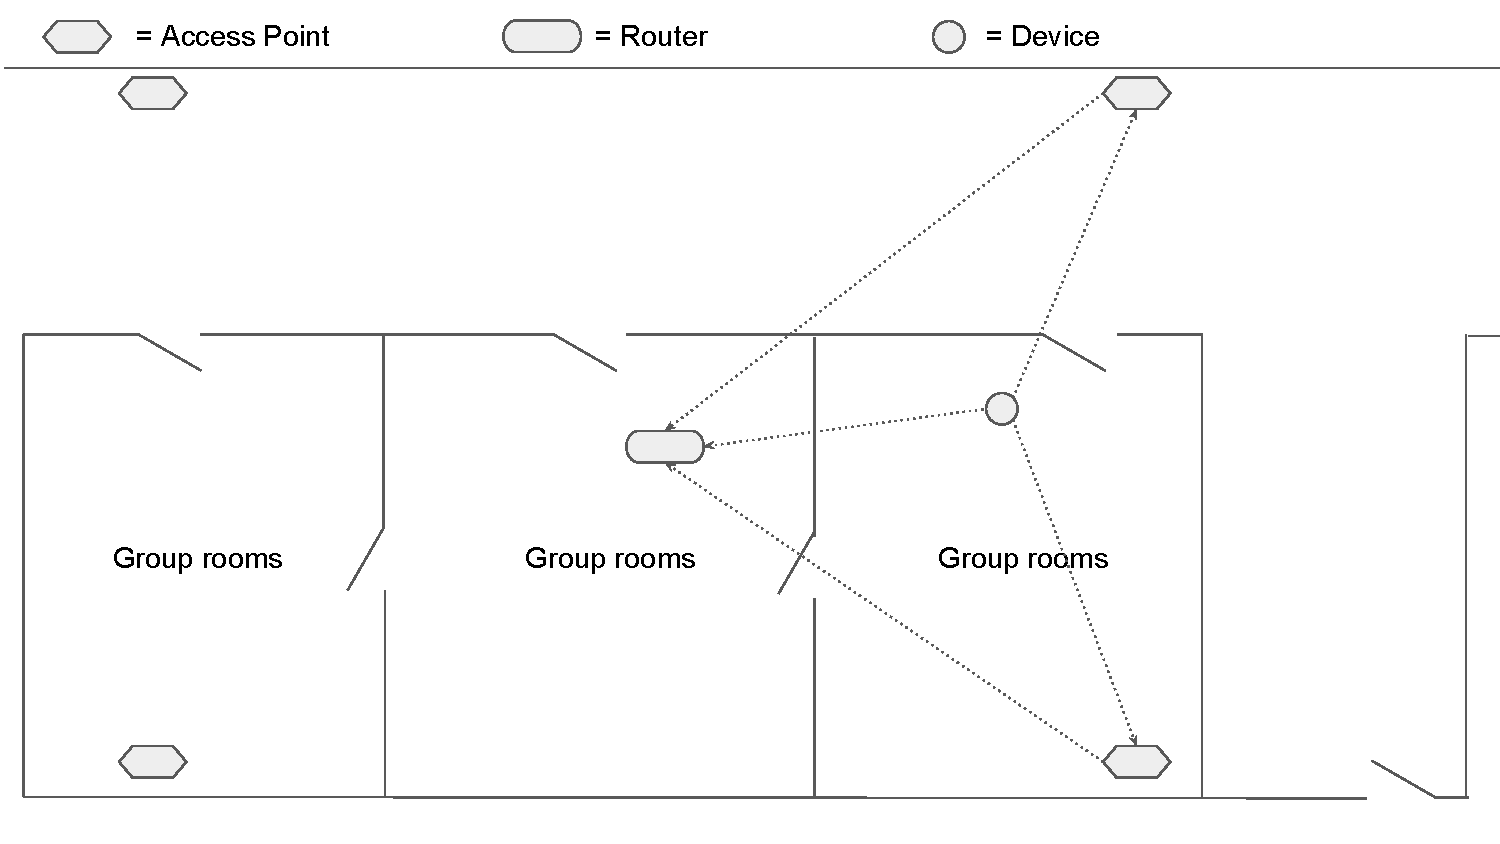
\includegraphics[scale=0.5]{graphics/Router-AccessPoint_Setup.pdf}
	\label{fig:OwnSetup}
	\caption{Illustration of how a positioning system can be set up, using routers and access point that can track devices.}
\end{figure}

\subsection*{Equipment Requirements}
The initial requirements for the equipment, is a wireless antenna capable of supporting 2.4 GHz and optionally 5 GHz. It would be advantageously if we set up two different ILBS for the sake of comparison. We decided to buy two brands allowing us to analyse at least two ILBS and thus conclude which of the systems performed best, based on the criteria describe in section \ref{sec:monitoring}.

Based on the above requirement we found two brands, Ubiquiti and D-link which in comparison is considered the cheaper brand. We ordered one router, two expensive and five cheap access points of each brand.

\subsection*{Access point positioning}\ofx{we may want to move this?}
Cisco\cite{access_point_placement} have guidelines for how to place the access points in order to get the best coverage for your system. They recommend that there are placed an access point in each corner of the building and some along the perimeter, in addition if the building is large enough there should be placed some within the perimeter that can form a sub-perimeter inside which there may be additional access points, this is illustrated in \cref{access_placement} on which the red circles are access points. This means the perimeter established by the outer most access points should encapsulate the entire floor. Everything on this perimeter is called the \textit{hull}\cite{access_point_placement}.

Each access point should be place 50-70 feet away from each other in order to get a high precision without a lot of unnecessary overlap\cite{access_point_range}.
 
The placement of the access points in \cref{fig:OwnSetup} is based on this design. As it can be seen they are placed in a square to symbolize corners and the router in the middle, in our small system.

\begin{figure}[H]
	\centering
	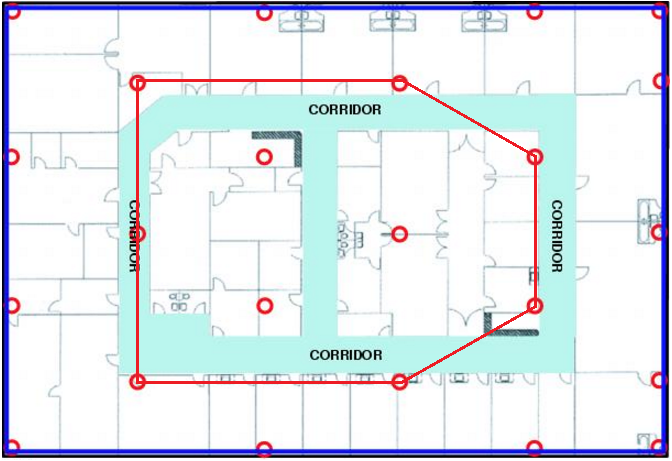
\includegraphics[scale=0.5]{graphics/access_placement.png}
	\label{fig:access_placement}
	\caption{Illustration of how access points should be placed.}
\end{figure}

\subsection*{Test Capabilities of the Equipment}
We tested the Ibiquiti equipment, with the original firmware. At first glance we are able to get transmission(TX) and receive(RX) signals of connected devices, unfortunately we do not receive the signals from devices not connected to the router. It was attempted to use the routers terminal which did not yield any results due to restricted access.

This caused us to research custom firmware for the router. By installing new firmware on the router we will be able to get root access to the router and thereby manipulate it at a lower level than the routers original firmware allows, this is necessary if we are to capture every receive signal the router gets.

We did find a custom firmware for Ibiquiti, however not for D-link. The searched sites were: openwrt.org{cite?}, polarcloud.com\ofx{cite?}, dd-wrt.com, gargolye-router.com\ofx{cite?}, librecmc.org\ofx{cite?} and wrtrouters.com\ofx{cite?}. These sites covers thousands of routers and the fact that we were not able to find a custom firmware for D-link might be because that the particular model we ordered\ofx{something is missing} because other routers from the same brand is supported. No conclusion was found, to why it is not covered on any of the websites.

We ended up utilizing the openwrt because it supports our Ibiquiti router and allows us to gain root access and execute programs. With the new custom firmware installed we have about 8Mb of memory left on the router, this put some limitations to which language we can use, our first attempt is to use a version of python called mini-python that dose not exceed the memory limit.

A program is constructed allowing us to listen on different types of networks such as LAN and WAN, this is done using the socket library. We were however not able to import the socket library which was required, to run our program on the router.
\section{Security considerations}\label{sec:secure}
In order to increase the level of security in our system, different considerations should be made. These considerations are made in order to make it more difficult for intruders to break into the system as well as protect sensitive information. We limit the discussion to program communication and the way sensitive information is handled, as this is the most sensitive part of the system. It would also improve the robustness of the system if these parts were made secure, as these are the parts of the program where it is possible to introduce erroneous, dirty data.

\subsection*{Certificates}
Certificates are used when communicating over the HTTPS protocol as a way to ensure the identity of a website as well as hand out the public key and encryption method. Once a certificate for a website is downloaded to a computer, the identity of the website can be verified against this certificate on subsequent visits. All communication with MSE uses the HTTPS protcol, and as such we have to consider how we treat certificates. 

Initially we created an empty certificate-handler which is still in use. This means that the identity of a website is accepted no matter what, potentially allowing for scam websites to copy the certificate and alter it slightly to pose as another website. An alternative, more secure solution, would be to download the certificates MSE uses and insert them in the JVM keystore, which is a collection of all accepted certificates. By freely accepting all certificates it is possible for attackers to input dirty data in the system by adding a server pretending to be an MSE service.

\subsection*{HTTPS}
The system currently communicates internally over HTTP, an insecure communication protocol that uses cleartext to communicate. Anybody intercepting the communication can read it with ease. We can diminish the damage from this type of attack by using the HTTPS protocol, short for \textit{Hyper Text Transfer Protocol Secure}, which functions as the HTTP protocol with the exception that the message is encrypted. This means that if someone were to gain access to the connection, they would not be able to read the information. A secure connection is very important on sites that handle sensitive information such as CPR-numbers or credit card data and this can be achieved by using the HTTPS protocol \cite{HTTPS}.

\begin{figure}[ht]
	\begin{center}
		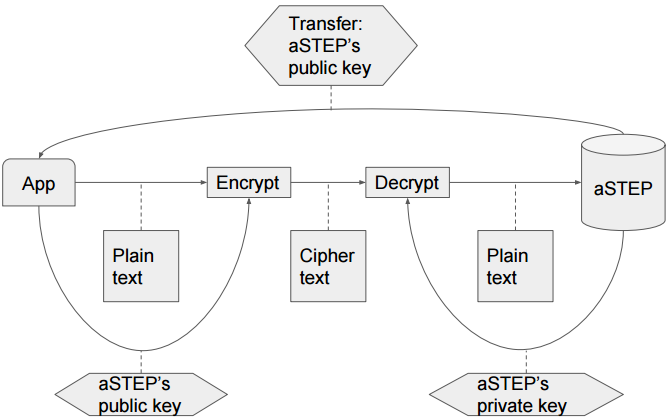
\includegraphics[scale=0.9]{graphics/encrypt_decrypt.png}
		\caption{HTTPS.}
		\label{fig:HTTPS}
	\end{center} 
\end{figure}

\Cref{fig:HTTPS} shows how HTTPS is used. In this example an app is sending data to the aSTEP server via the HTTPS protocol. First the app retrieves aSTEP's public key from the downloaded certificate. This public key is then used to encrypt all the data that is going to be sent to aSTEP. When aSTEP receives the data, the private key is used to decrypt the data, which can then be read as plain text. Additionally, if aSTEP needs to send data back to the app, it will need the apps public key to encrypt the message and the app will use its own private key to decrypt the data \cite{HTTPS}.

\subsection*{Hashing}
Hash functions are most commonly used to store a users password or other sensitive data. It functions as a one way mapping; when a message is hashed it can not be reversed again. The formal definition is shown below:
\begin{quote}
\textit{'A hash function is a computationally efficient function mapping binary strings of arbitrary length to binary strings of some fixed length, called hash-values.' \cite{Hash_def}}
\end{quote}

It has been requested by the Heatmap application group to have a unique identification of all people. As we are not allowed to store the MAC address, a solution to this would be to hash the MAC address with a random, changing salt. In this way it will be possible for the application to track people for as long as the salt-value is unchanged.

\begin{figure}[ht]
	\begin{center}
		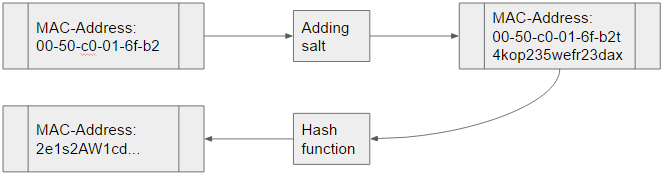
\includegraphics[scale=0.9]{graphics/salt.png}
		\caption{salting and hashing a MAC Address.}
		\label{fig:salt}
	\end{center} 
\end{figure}

\Cref{fig:salt} illustrates how a MAC address is first salted and then hashed.

Java has a hash-method implemented in the object class called \textit{hashCode()}, this may be used for hashing information. When using a hash function, you add a randomly generated string that extends the original message. The generated string is called a salt and makes the hash function more secure.

\subsection*{Hard-coded Passwords}
When communicating with MSE from the intermediate server as well as when communicating with the intermediate server, we are currently using hard-coded passwords. This means that everyone with access to the code can find the log-in information. The information should be given as arguments to the program and hashed such that the log-in can not be seen in the code and cannot be read as plain text in memory. 

%\subsection*{Visibility}
%As of now many parts of the system has a higher degree of visibility than necessary. This makes it possible to use functionality in unexpected ways and possibly cause unintended behaviour. We can decrease the level of visibility by having private and protected classes and methods, which leads to a system that is more resilient towards unexpected usage.
 
\subsection*{Obfuscating Personal Information}
In order to ensure our users personal information, we decided to obfuscate the e-mail addresses. By doing so there will be no way for outsiders to identify people unwilling to have their information stored.

IP addresses are not considered personal information. This is based on the fact that the address changes each time you change access point. By not obfuscating the IP address, applications will be able to see how many people are connected to a given access point. This can be done by identifying the first 16 bits for IPv4 or the first 48 bits for IPv6, also known as the netbits \cite{IPnetworkID}.

\section{Sprint Evaluation}
To perform an evaluation of the sprint we iterate over the sprint goals and comment on whether or not they were fulfilled.

During this sprint we examined the possibility of building a small tracking system utilising access points. The goal was to have a system that is comparable with MSE in terms of the precision of the geographical coordinates. We were not able to make a functional IPS as we were unable to retrieve the RSSI from the routers and access points. \Cref{sec:futureSystem} will function as a guidance and proposal section for how to continue the development of the system.

We deployed an update for the intermediate service communicating with MSE, fixing several issues and creating support for geographical coordinates opposed to the relative once we got before. The update was successfully installed and deployed. This concludes our shortcomings from \cref{cha:sprint2}.

The security considerations lead us to be wary of different security pitfalls and sensitive areas of the system. We have made some decisions regarding what information to obfuscate and what information to keep. It was decided to obfuscate the MAC address and e-mail, by hashing the MAC address and deleting the e-mail address.